\documentclass[14pt]{extbook}
\usepackage{multicol, enumerate, enumitem, hyperref, color, soul, setspace, parskip, fancyhdr} %General Packages
\usepackage{amssymb, amsthm, amsmath, latexsym, units, mathtools} %Math Packages
\everymath{\displaystyle} %All math in Display Style
% Packages with additional options
\usepackage[headsep=0.5cm,headheight=12pt, left=1 in,right= 1 in,top= 1 in,bottom= 1 in]{geometry}
\usepackage[usenames,dvipsnames]{xcolor}
\usepackage{dashrule}  % Package to use the command below to create lines between items
\newcommand{\litem}[1]{\item#1\hspace*{-1cm}\rule{\textwidth}{0.4pt}}
\pagestyle{fancy}
\lhead{Progress Quiz 10}
\chead{}
\rhead{Version C}
\lfoot{5170-5105}
\cfoot{}
\rfoot{Summer C 2021}
\begin{document}

\begin{enumerate}
\litem{
Which of the following equations \textit{could} be of the graph presented below?
\begin{center}
    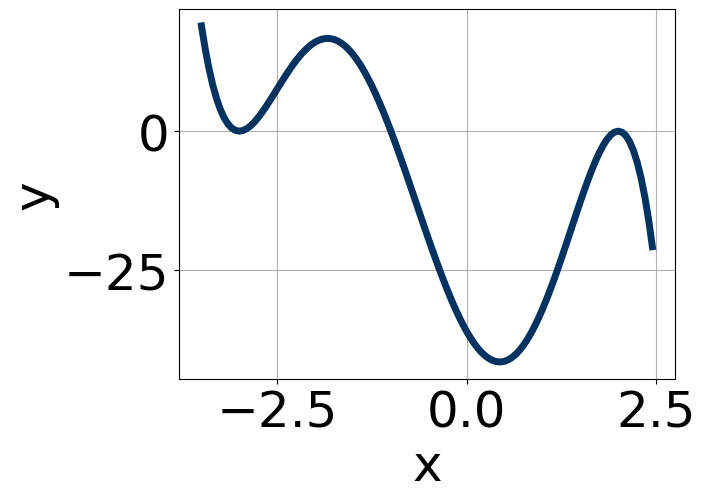
\includegraphics[width=0.5\textwidth]{../Figures/polyGraphToFunctionC.png}
\end{center}
\begin{enumerate}[label=\Alph*.]
\item \( 19(x - 2)^{10} (x + 3)^{6} (x + 1)^{8} \)
\item \( -18(x - 2)^{10} (x + 3)^{6} (x + 1)^{11} \)
\item \( -19(x - 2)^{8} (x + 3)^{9} (x + 1)^{10} \)
\item \( 13(x - 2)^{10} (x + 3)^{10} (x + 1)^{5} \)
\item \( -4(x - 2)^{10} (x + 3)^{5} (x + 1)^{5} \)

\end{enumerate} }
\litem{
Describe the end behavior of the polynomial below.\[ f(x) = 4(x + 6)^{4}(x - 6)^{9}(x + 9)^{3}(x - 9)^{3} \]\begin{enumerate}[label=\Alph*.]
\begin{multicols}{2}\item 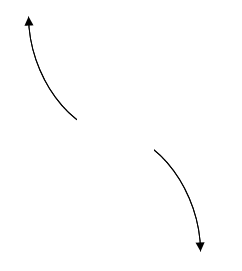
\includegraphics[width = 0.3\textwidth]{../Figures/polyEndBehaviorAC.png}\item 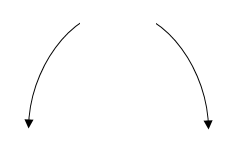
\includegraphics[width = 0.3\textwidth]{../Figures/polyEndBehaviorBC.png}\item 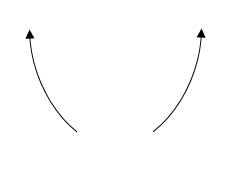
\includegraphics[width = 0.3\textwidth]{../Figures/polyEndBehaviorCC.png}\item 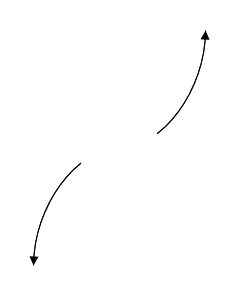
\includegraphics[width = 0.3\textwidth]{../Figures/polyEndBehaviorDC.png}\end{multicols}\item None of the above.
\end{enumerate} }
\litem{
Construct the lowest-degree polynomial given the zeros below. Then, choose the intervals that contain the coefficients of the polynomial in the form $x^3+bx^2+cx+d$.\[ -3 - 5 i \text{ and } -4 \]\begin{enumerate}[label=\Alph*.]
\item \( b \in [-1, 5], c \in [8, 9.7], \text{ and } d \in [16, 22] \)
\item \( b \in [-1, 5], c \in [6.7, 8.6], \text{ and } d \in [10, 14] \)
\item \( b \in [-15, -8], c \in [56.1, 58.3], \text{ and } d \in [-143, -134] \)
\item \( b \in [6, 14], c \in [56.1, 58.3], \text{ and } d \in [130, 141] \)
\item \( \text{None of the above.} \)

\end{enumerate} }
\litem{
Which of the following equations \textit{could} be of the graph presented below?
\begin{center}
    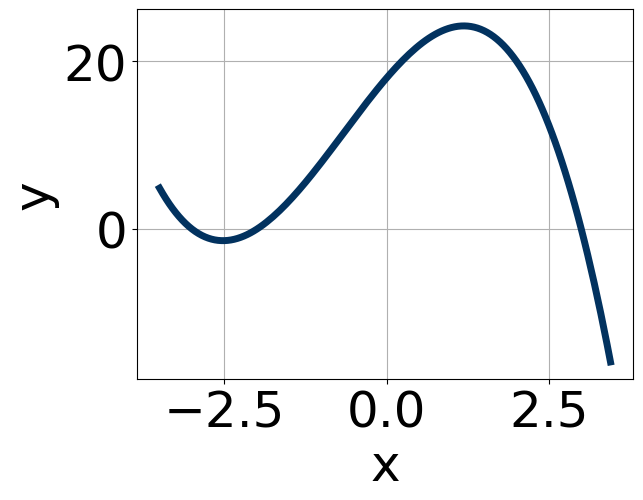
\includegraphics[width=0.5\textwidth]{../Figures/polyGraphToFunctionCopyC.png}
\end{center}
\begin{enumerate}[label=\Alph*.]
\item \( 7(x + 2)^{6} (x + 3)^{11} (x - 3)^{7} \)
\item \( -10(x + 2)^{10} (x + 3)^{9} (x - 3)^{9} \)
\item \( 11(x + 2)^{9} (x + 3)^{9} (x - 3)^{9} \)
\item \( -2(x + 2)^{9} (x + 3)^{11} (x - 3)^{5} \)
\item \( -5(x + 2)^{4} (x + 3)^{8} (x - 3)^{9} \)

\end{enumerate} }
\litem{
Describe the zero behavior of the zero $x = -6$ of the polynomial below.\[ f(x) = -9(x - 6)^{9}(x + 6)^{10}(x + 2)^{9}(x - 2)^{12} \]\begin{enumerate}[label=\Alph*.]
\begin{multicols}{2}\item 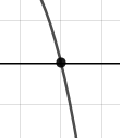
\includegraphics[width = 0.3\textwidth]{../Figures/polyZeroBehaviorCopyAC.png}\item 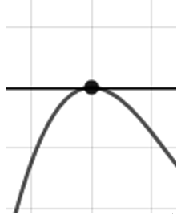
\includegraphics[width = 0.3\textwidth]{../Figures/polyZeroBehaviorCopyBC.png}\item 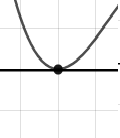
\includegraphics[width = 0.3\textwidth]{../Figures/polyZeroBehaviorCopyCC.png}\item 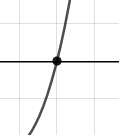
\includegraphics[width = 0.3\textwidth]{../Figures/polyZeroBehaviorCopyDC.png}\end{multicols}\item None of the above.
\end{enumerate} }
\litem{
Construct the lowest-degree polynomial given the zeros below. Then, choose the intervals that contain the coefficients of the polynomial in the form $ax^3+bx^2+cx+d$.\[ -2, \frac{-7}{3}, \text{ and } \frac{3}{2} \]\begin{enumerate}[label=\Alph*.]
\item \( a \in [5, 11], b \in [16, 20], c \in [-14, -9], \text{ and } d \in [40, 47] \)
\item \( a \in [5, 11], b \in [-12, -2], c \in [-33, -27], \text{ and } d \in [40, 47] \)
\item \( a \in [5, 11], b \in [-43, -32], c \in [63, 68], \text{ and } d \in [-47, -37] \)
\item \( a \in [5, 11], b \in [-21, -14], c \in [-14, -9], \text{ and } d \in [40, 47] \)
\item \( a \in [5, 11], b \in [16, 20], c \in [-14, -9], \text{ and } d \in [-47, -37] \)

\end{enumerate} }
\litem{
Construct the lowest-degree polynomial given the zeros below. Then, choose the intervals that contain the coefficients of the polynomial in the form $x^3+bx^2+cx+d$.\[ -4 - 3 i \text{ and } -3 \]\begin{enumerate}[label=\Alph*.]
\item \( b \in [11, 19], c \in [48.36, 49.78], \text{ and } d \in [72.6, 77.1] \)
\item \( b \in [0, 7], c \in [4.02, 6.83], \text{ and } d \in [7.9, 9.5] \)
\item \( b \in [0, 7], c \in [6.29, 9.06], \text{ and } d \in [11.8, 14.7] \)
\item \( b \in [-16, -10], c \in [48.36, 49.78], \text{ and } d \in [-76, -71.8] \)
\item \( \text{None of the above.} \)

\end{enumerate} }
\litem{
Construct the lowest-degree polynomial given the zeros below. Then, choose the intervals that contain the coefficients of the polynomial in the form $ax^3+bx^2+cx+d$.\[ \frac{-7}{5}, \frac{-1}{4}, \text{ and } \frac{3}{5} \]\begin{enumerate}[label=\Alph*.]
\item \( a \in [100, 104], b \in [-230, -224], c \in [129, 136], \text{ and } d \in [-21, -15] \)
\item \( a \in [100, 104], b \in [-177, -171], c \in [30, 38], \text{ and } d \in [20, 32] \)
\item \( a \in [100, 104], b \in [-112, -104], c \in [-65, -60], \text{ and } d \in [20, 32] \)
\item \( a \in [100, 104], b \in [103, 115], c \in [-65, -60], \text{ and } d \in [20, 32] \)
\item \( a \in [100, 104], b \in [103, 115], c \in [-65, -60], \text{ and } d \in [-21, -15] \)

\end{enumerate} }
\litem{
Describe the zero behavior of the zero $x = 7$ of the polynomial below.\[ f(x) = -7(x - 3)^{11}(x + 3)^{9}(x - 7)^{14}(x + 7)^{9} \]\begin{enumerate}[label=\Alph*.]
\begin{multicols}{2}\item 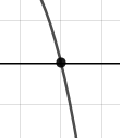
\includegraphics[width = 0.3\textwidth]{../Figures/polyZeroBehaviorAC.png}\item 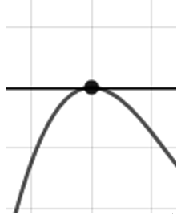
\includegraphics[width = 0.3\textwidth]{../Figures/polyZeroBehaviorBC.png}\item 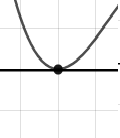
\includegraphics[width = 0.3\textwidth]{../Figures/polyZeroBehaviorCC.png}\item 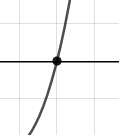
\includegraphics[width = 0.3\textwidth]{../Figures/polyZeroBehaviorDC.png}\end{multicols}\item None of the above.
\end{enumerate} }
\litem{
Describe the end behavior of the polynomial below.\[ f(x) = -3(x + 9)^{5}(x - 9)^{8}(x - 3)^{2}(x + 3)^{3} \]\begin{enumerate}[label=\Alph*.]
\begin{multicols}{2}\item 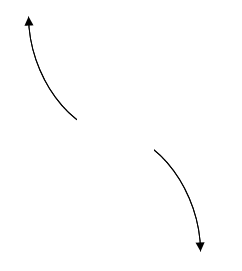
\includegraphics[width = 0.3\textwidth]{../Figures/polyEndBehaviorCopyAC.png}\item 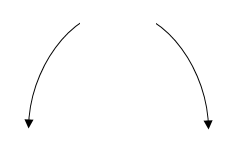
\includegraphics[width = 0.3\textwidth]{../Figures/polyEndBehaviorCopyBC.png}\item 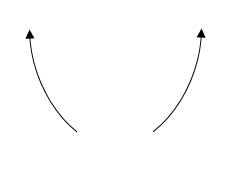
\includegraphics[width = 0.3\textwidth]{../Figures/polyEndBehaviorCopyCC.png}\item 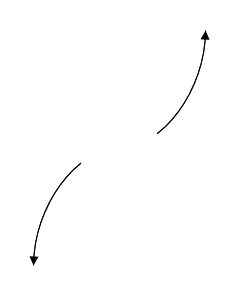
\includegraphics[width = 0.3\textwidth]{../Figures/polyEndBehaviorCopyDC.png}\end{multicols}\item None of the above.
\end{enumerate} }
\end{enumerate}

\end{document}